% !TEX program = pdflatex
\documentclass[aspectratio=169, 11pt]{beamer}

\usetheme{default}
\usecolortheme{default}
\setbeamertemplate{navigation symbols}{}
\setbeamertemplate{footline}[frame number]
\setbeamertemplate{frametitle}{\vspace{0.5em}\textbf{\insertframetitle}}

\usepackage{amsmath,amssymb}
\usepackage{graphicx}
\usepackage{booktabs}
\usepackage{colortbl}
\usepackage{xcolor}
\usepackage{pgfpages}

\setbeameroption{show notes on second screen=right}

\graphicspath{{../}}

\definecolor{resultbg}{HTML}{E8F5E9}
\definecolor{newbg}{HTML}{FFF9C4}
\definecolor{proofbg}{HTML}{E3F2FD}

\title{Week 3 Update}
\author{Michael Fang}
\date{March 2026}

\begin{document}

%----------------------------------------------------------------------
\begin{frame}
\centering
\vspace{2em}
{\Large\textbf{Week 3 Update}}

\vspace{1em}
Michael Fang

\vspace{0.5em}
March 2026
\end{frame}
\note{
Six main investigations from the meeting, plus some extensions.
The central surprise: the 2<alpha<3 gap can only be filled by
non-unimodular matrices --- a first example was found.
}

%----------------------------------------------------------------------
\begin{frame}{Recap and plan for this week}

\begin{columns}[T]
\begin{column}{0.48\textwidth}
Where we left off:
\vspace{0.3em}
\small
\begin{tabular}{llcc}
\toprule
\textbf{Pattern} & \textbf{Cl.} & $\alpha$ & $\bar\Lambda$ \\
\midrule
Integer Lattice     & I   & $\infty$ & $1/6$ \\
Fibonacci           & I   & 3        & 0.201 \\
Silver              & I   & 3        & 0.250 \\
Bronze--Nickel      & I   & 3        & 0.282--0.310 \\
URL ($a=1$)         & I   & 2        & $1/3$ \\
Stealthy $\chi=0.3$ & I   & ---      & 0.357 \\
Bombieri-Taylor     & I   & 1.545    & 0.377 \\
\midrule
Period-Doubling     & II  & 1        & div. \\
0222 chain          & III & 0.64     & div. \\
\bottomrule
\end{tabular}
\end{column}
\begin{column}{0.50\textwidth}
Questions from the meeting:
\begin{itemize}
  \item Spreadability gives $\hat\alpha\approx1.9$ for BT, not 1.545 --- why?
  \item How do estimates converge with $N$?
  \item Can we fill the $2<\alpha<3$ gap with a substitution chain?
  \item What plays the role of $\bar\Lambda$ for Classes II and III?
  \item Does $\bar\Lambda$ have a finite-$N$ correction?
  \item Stealthy: is $\alpha$ well-defined? Are densities comparable?
\end{itemize}
\end{column}
\end{columns}
\end{frame}
\note{
The metallic-mean chains all give alpha=3 because the 2x2 det=1 constraint forces
|lambda_2| = 1/lambda_1.  BT breaks this with a 3x3 matrix.
Stealthy: S(k)=0 over a finite k-interval by design, not a power law -- alpha=infinity is misleading.
URL cloaked Lambda-bar=1/3 exact from Klatt et al. 2020.
}

%----------------------------------------------------------------------
\begin{frame}{Why spreadability fails for Bombieri-Taylor}

\begin{columns}[T]
\begin{column}{0.56\textwidth}
\centering

\includegraphics[width=\linewidth]{figures/fig_bt_deep.png}
\end{column}
\begin{column}{0.42\textwidth}
Two things go wrong simultaneously.

\medskip
\textbf{Dense Bragg spectrum.}
BT has 32,517 Bragg peaks in $k<50$
(12$\times$ more than Fibonacci).
The spreadability $\mathcal{S}(t)$ oscillates
log-periodically with period $2\ln\theta_1\approx1.62$,
masking any power-law decay.

\medskip
\textbf{Large sub-leading eigenvalue.}
$|\lambda_2|=0.802$ for BT vs.\ 0.618 for Fibonacci.
The oscillations die out very slowly.
Even over $t\in[10^5,10^9]$, the fit gives
$\hat\alpha=1.67$ instead of 1.545.

\medskip
\colorbox{resultbg}{\parbox{0.96\linewidth}{
  $\bar\Lambda$ from $\sigma^2(R)$ works fine: it averages
  over these oscillations.
  $\bar\Lambda=0.377$, stable from $N\sim2000$.
}}
\end{column}
\end{columns}
\end{frame}
\note{
Rod overlap also matters: minimum BT inter-point spacing = 1.000; need 2a < 1.000; corrected
rod radius to a=0.45.
The variance-based Lambda-bar is robust because it's a running average over R, so the
log-periodic oscillations cancel.
Conclusion: use Lambda-bar (not spreadability) for any quasicrystal with large |lambda_2|.
}

%----------------------------------------------------------------------
\begin{frame}{How well do our estimates converge with $N$?}

\begin{columns}[T]
\begin{column}{0.57\textwidth}
\centering
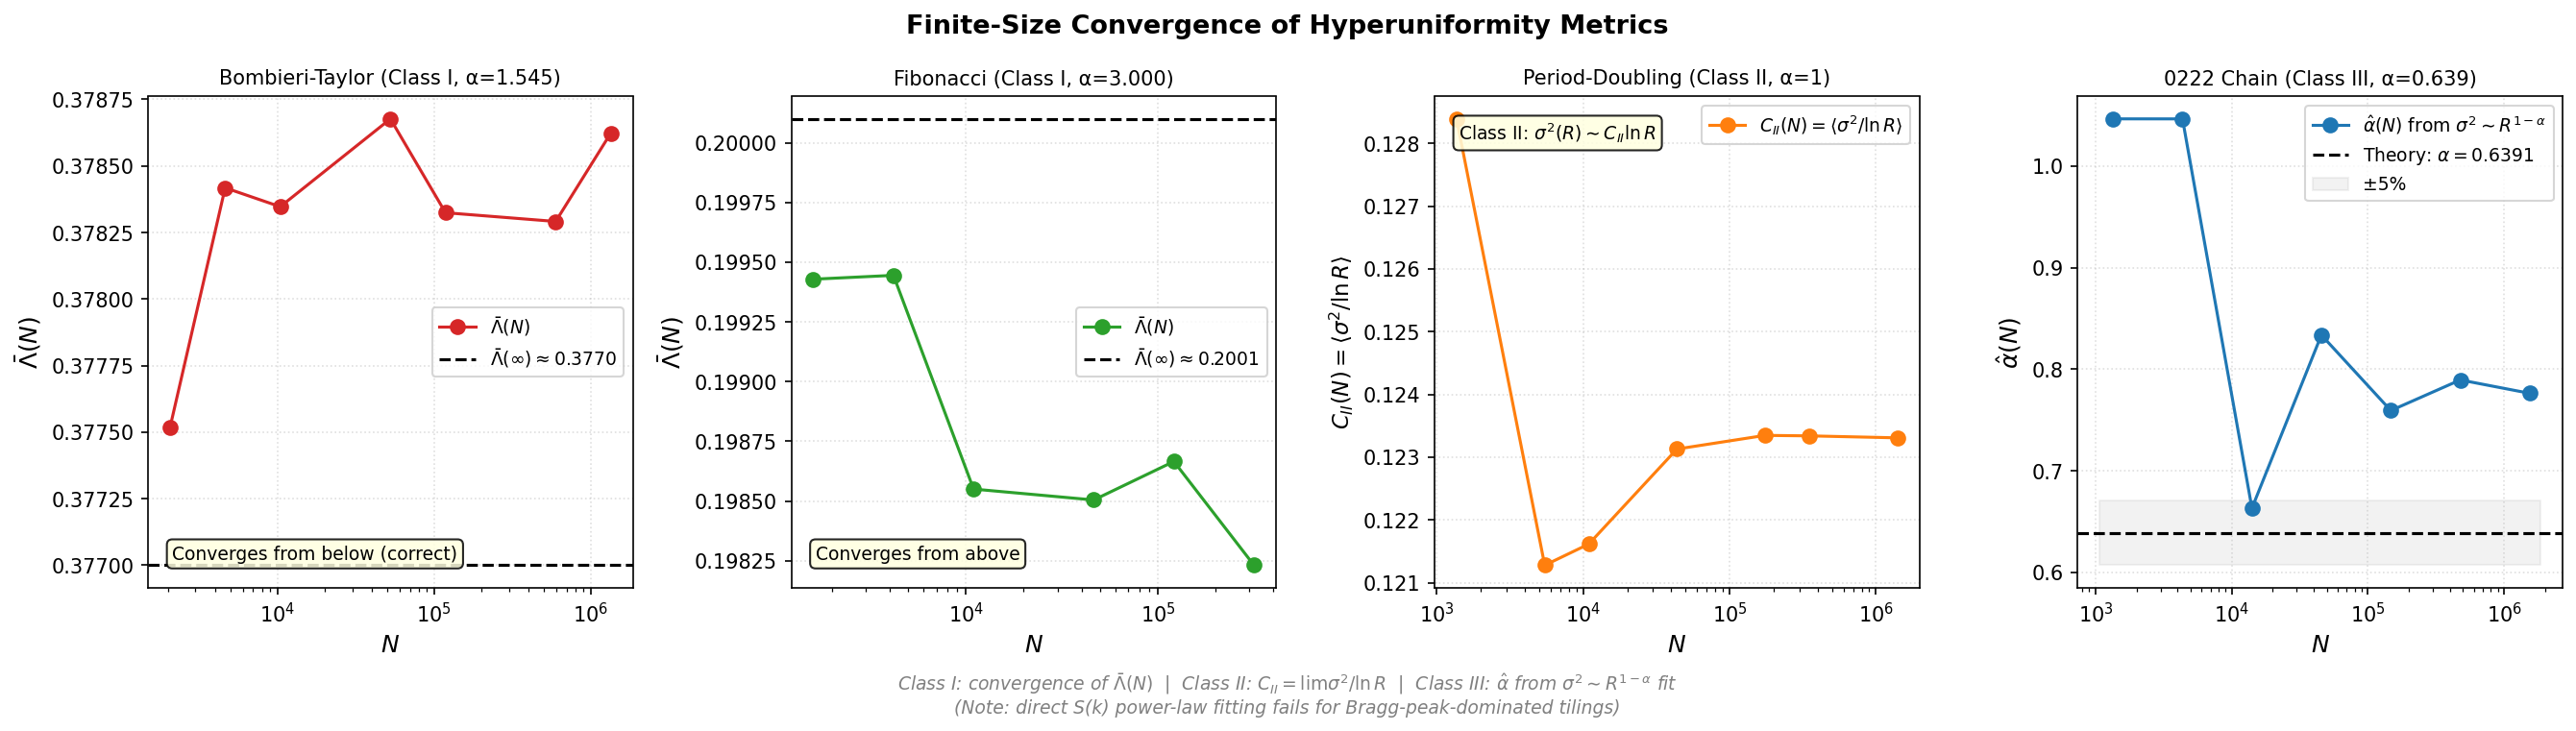
\includegraphics[width=\linewidth]{figures/fig_finite_size_alpha_landscape.png}
\end{column}
\begin{column}{0.41\textwidth}
\small
\begin{tabular}{lcc}
\toprule
\textbf{Pattern} & $N\!\sim\!10^3$ & $N\!\sim\!10^6$ \\
\midrule
BT\ \ $\bar\Lambda$   & 0.378 & 0.379 \\
Fib.\ $\bar\Lambda$   & 0.199 & 0.198 \\
PD\ \ $C_{II}$        & 0.128 & 0.123 \\
0222 $\hat\alpha$     & 1.05  & 0.78  \\
\bottomrule
\end{tabular}

\vspace{0.8em}
Key takeaways:
\begin{itemize}
  \item Fitting $S(k)\sim k^\alpha$ directly fails ---
    substitution tilings have Bragg peaks, not a smooth background
  \item Class~I $\bar\Lambda$ is stable from $N\sim1000$
  \item Class~III is slow because $|\lambda_2|=1.24>1$
    (not Pisot, diffuse spectrum)
\end{itemize}
\end{column}
\end{columns}
\end{frame}
\note{
S(k) for a substitution tiling = superposition of delta functions at Bragg positions.
There is no smooth k^alpha background to fit.
0222 chain: |lambda_2| = sqrt(5)-1 ~ 1.236 > 1; not a Pisot number, so S(k) has a diffuse
component and alpha-hat oscillates widely across N values.
Class I Lambda-bar is a spatial average: big fluctuations at individual R values cancel
when averaged, giving stable convergence from N~1000.
}

%----------------------------------------------------------------------
\begin{frame}{Searching for a $2<\alpha<3$ quasicrystal}

\begin{columns}[T]
\begin{column}{0.50\textwidth}
\centering
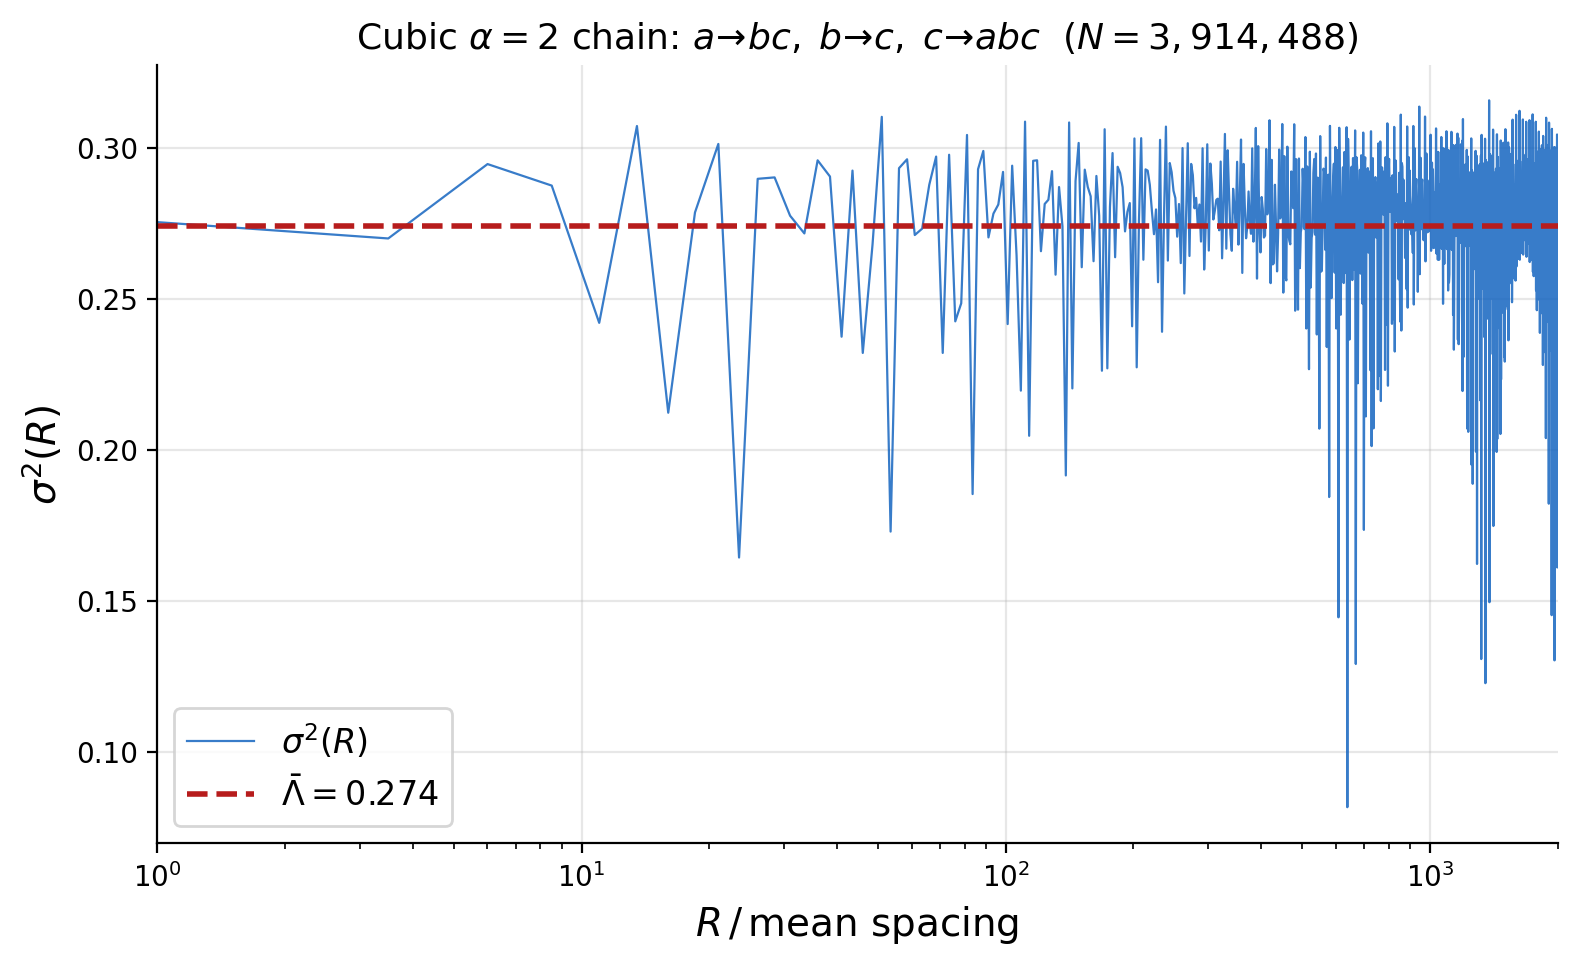
\includegraphics[width=\linewidth]{figures/fig_new_tilings.png}
\end{column}
\begin{column}{0.48\textwidth}
I enumerated all $3\times3$ substitution matrices with row sums $\leq4$:
\[
  39{,}304\ \xrightarrow{\text{Pisot}}\ 4{,}882
  \ \xrightarrow{\text{target}\ \alpha\in(2,3)}\ 305
\]
\colorbox{newbg}{All 305 give $\alpha=2$ or $\alpha=3$. The gap is empty.}

\medskip
This is not a coincidence.
For any $3\times3$ unimodular matrix with a complex eigenvalue pair:
\[
  \underbrace{\det M}_{=1} = \lambda_1|\lambda_2|^2
  \;\Rightarrow\; |\lambda_2| = \frac{1}{\sqrt{\lambda_1}}
  \;\Rightarrow\; \alpha = 2
\]
For all-real sub-leading eigenvalues, the search finds only $\alpha=3$.
\end{column}
\end{columns}
\end{frame}
\note{
The Pisot condition requires all sub-leading eigenvalues to have |lambda_i| < 1 (pure Bragg
diffraction); non-Pisot matrices give diffuse spectra.
The complex-pair identity: det M = lambda_1 * lambda_2 * conj(lambda_2) = lambda_1 |lambda_2|^2.
For det=1: |lambda_2| = 1/sqrt(lambda_1) EXACTLY, regardless of the specific lambda_1.
This pins alpha=2 for every 3x3 unimodular matrix with a complex pair.
}

%----------------------------------------------------------------------
\begin{frame}{A new deterministic substitution tiling at $\alpha=2$}

A nice byproduct of the search.
\medskip

\begin{columns}[T]
\begin{column}{0.48\textwidth}
\textbf{Substitution:}\; $a\!\to\!bc,\; b\!\to\!c,\; c\!\to\!abc$
\[
  M = \begin{pmatrix}0&1&1\\0&0&1\\1&1&1\end{pmatrix},\quad
  |\det M| = 1
\]
$\lambda_1\approx2.148$,\; $|\lambda_{2,3}|\approx0.682$ (complex pair)
\[
  \alpha = 1 - \frac{2\ln(0.682)}{\ln(2.148)} = \textbf{2.000 (exact)}
\]
$\bar\Lambda=0.275$, Class~I, $N\approx1.8$ million points.
\end{column}
\begin{column}{0.50\textwidth}
Previously, only the URL reached $\alpha=2$ --- through random displacements
from an integer lattice. This is the first \emph{deterministic} quasiperiodic
substitution tiling with $\alpha=2$.

\vspace{0.8em}
\small
\begin{tabular}{lcc}
\toprule
\textbf{Pattern} & $\alpha$ & $\bar\Lambda$ \\
\midrule
Silver             & 3     & 0.250 \\
\rowcolor{newbg}
Cubic $\alpha{=}2$ & 2     & 0.275 \\
Bronze             & 3     & 0.282 \\
URL ($a=1$)        & 2     & 0.333 \\
\bottomrule
\end{tabular}

\vspace{0.5em}
$\bar\Lambda=0.275$ sits between Silver and Bronze.
\end{column}
\end{columns}
\end{frame}
\note{
Characteristic polynomial: x^3-x^2-2x-1=0.
Lambda_bar=0.275 lies between Silver (0.250) and Bronze (0.282).
Pattern generated to N~1.8 million points.
The alpha=2 value is exact by the algebraic argument: det=1 + complex pair -> alpha=2.
The URL achieves alpha=2 stochastically (independent random displacements); this chain
achieves it through a deterministic substitution rule.
}

%----------------------------------------------------------------------
\begin{frame}{Metrics for Classes II and III}

\begin{columns}[T]
\begin{column}{0.58\textwidth}
\centering
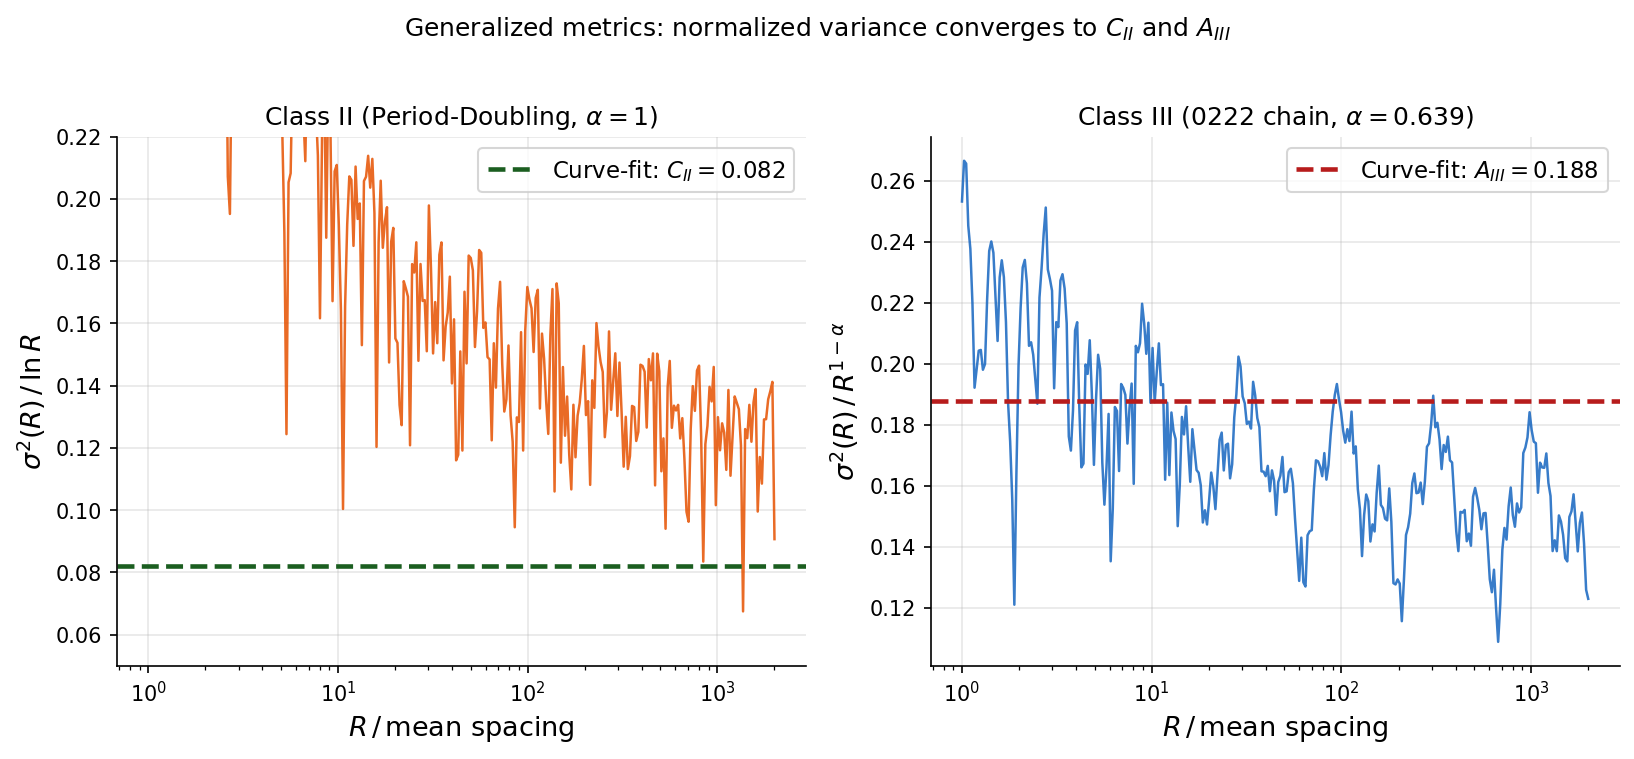
\includegraphics[width=\linewidth]{figures/fig_generalized_metrics.png}

\vspace{0.2em}
{\footnotesize Each normalized variance plateaus at large $R$, confirming the asymptotic scaling.}
\end{column}
\begin{column}{0.40\textwidth}
$\bar\Lambda$ diverges outside Class~I.
The natural generalizations:

\medskip
\textbf{Class II}\; ($\sigma^2\sim C_{II}\ln R$):
\[
  C_{II} = \lim_{R\to\infty}\frac{\sigma^2(R)}{\ln R}
\]
Period-Doubling: $C_{II} = 0.123\pm0.016$

\bigskip
\textbf{Class III}\; ($\sigma^2\sim A_{III}\,R^{1-\alpha}$):
\[
  A_{III} = \lim_{R\to\infty}\frac{\sigma^2(R)}{R^{1-\alpha}}
\]
0222 chain ($\alpha=0.639$): $A_{III} = 0.151\pm0.014$
\end{column}
\end{columns}
\end{frame}
\note{
Period-Doubling: |lambda_2|=1 exactly (alpha=1, boundary Pisot).
0222: |lambda_2| = sqrt(5)-1 > 1 (not Pisot), hence diffuse component.
C_II requires N > 100k to converge; A_III convergence is slow.
These have been added as compute_generalized_metric() in quasicrystal_variance.py.
}

%----------------------------------------------------------------------
\begin{frame}{$\bar\Lambda$ at finite $N$: lattice and stealthy}

\begin{columns}[T]
\begin{column}{0.54\textwidth}
\centering
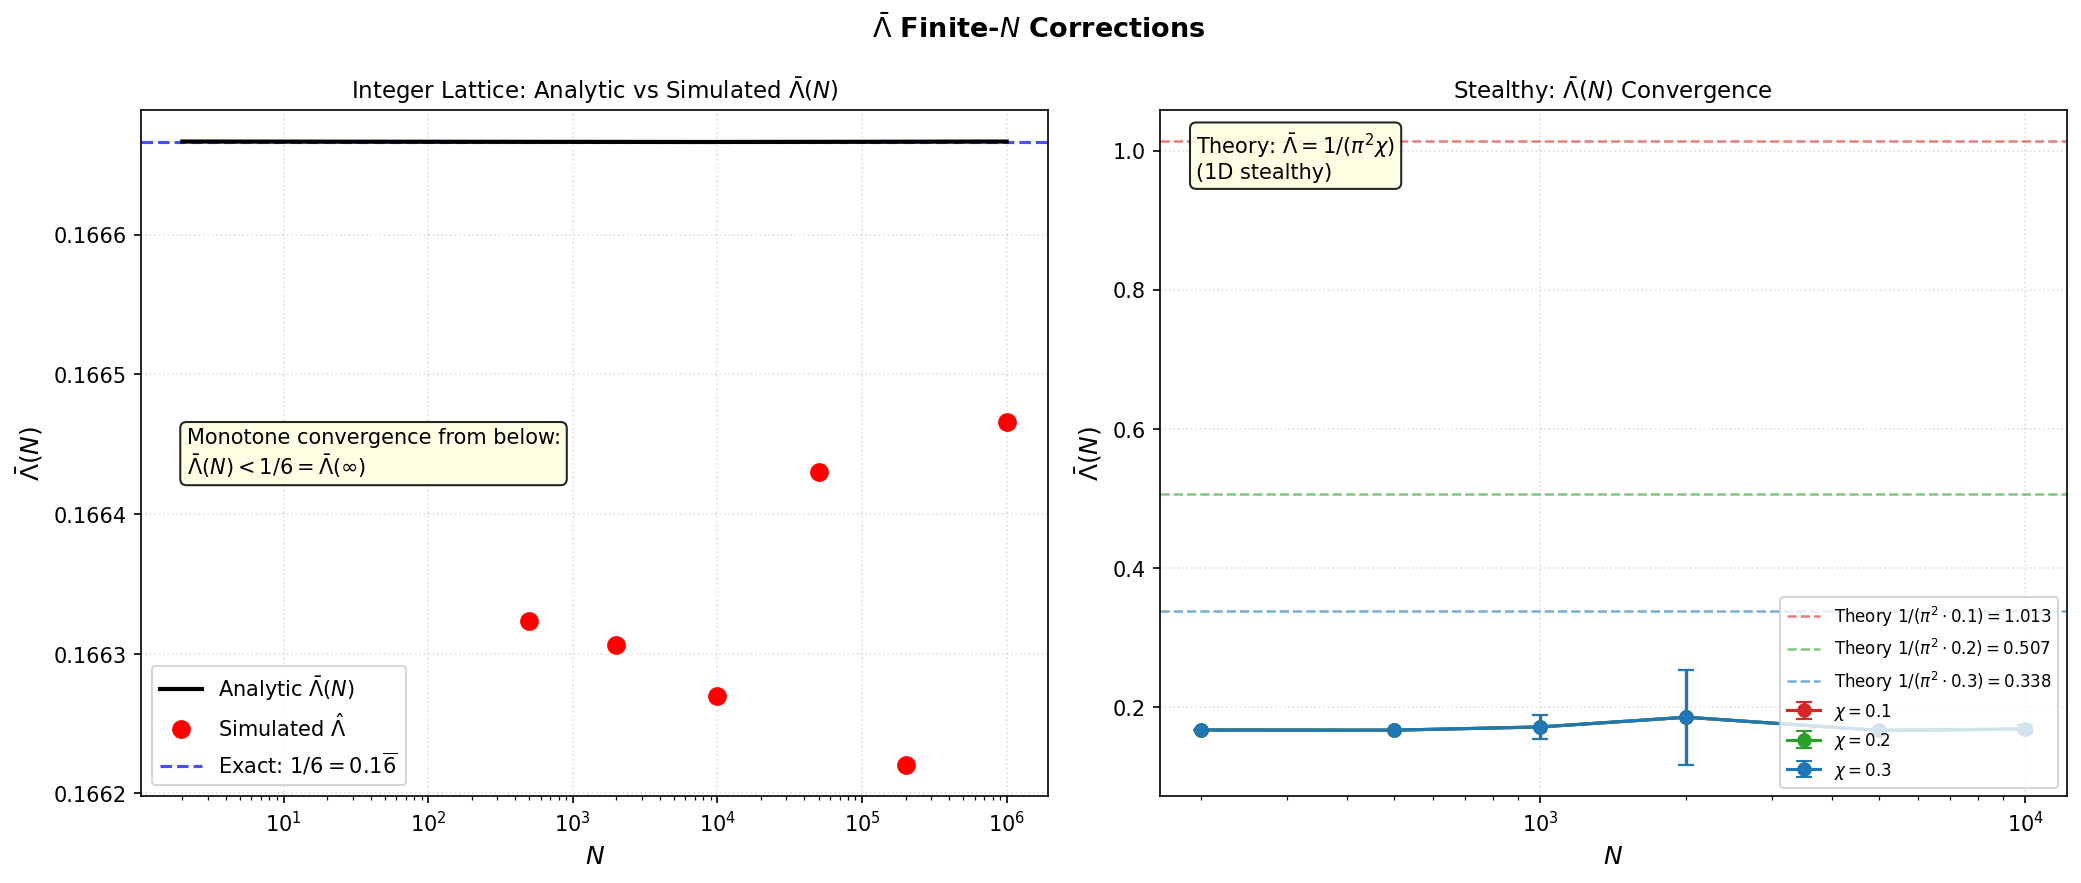
\includegraphics[width=\linewidth]{figures/fig_finite_size_lambda.png}
\end{column}
\begin{column}{0.44\textwidth}
\textbf{Integer lattice.}
$\sigma^2(R)=\{2R\}(1-\{2R\})$ exactly, so:
\[
  \bar\Lambda(R_\text{max}) = \tfrac{1}{6}
  \quad \text{for all integer}\ R_\text{max}
\]
No finite-$N$ correction at all.

\medskip
\textbf{Stealthy: two distinct phases.}

\vspace{0.3em}
\small
\begin{tabular}{lc}
\toprule
\textbf{Initial condition} & $\bar\Lambda$ \\
\midrule
Perturbed lattice  & $\approx 1/6$ \\
Random positions  & $1/(\pi^2\chi)$ \\
\bottomrule
\end{tabular}

\vspace{0.4em}
\normalsize
Both satisfy $S(k)=0$ for $|k|<K^*$.
They are genuinely different ground states
of the same optimization problem.
\end{column}
\end{columns}
\end{frame}
\note{
Lattice sigma^2(R) = {2R}(1-{2R}) integrates exactly to 1/12 over each half-period,
so the running average is always 1/6 at integer R_max.
Stealthy: starting from a perturbed lattice, the optimizer finds a near-lattice ground state
(Lambda_bar ~ 1/6).  Starting from random positions (collaborator data), it finds the
disordered phase (Lambda_bar = 1/(pi^2 chi)).
Key insight: stealthy hyperuniform configurations are highly non-unique.
}

%----------------------------------------------------------------------
\begin{frame}{Updated catalog}

\begin{columns}[T]
\begin{column}{0.50\textwidth}
\centering

\includegraphics[width=\linewidth]{figures/fig_catalog_updated.png}
\end{column}
\begin{column}{0.48\textwidth}
Two corrections from this week:

\medskip
\textbf{Stealthy reclassified.}
Reporting $\alpha=\infty$ for stealthy patterns
is misleading: $S(k)=0$ is a design constraint,
not a power-law suppression.
Now described by $\chi$ and $K^*=2\pi\rho\chi$.

\medskip
\textbf{Density comparison is valid.}
$\bar\Lambda$ is invariant under density rescaling
$x_i\to x_i/\rho$ in $d=1$ (verified numerically,
difference $<0.001$).
Direct $\bar\Lambda$ comparisons across all patterns
are fine.

\medskip
\small
\begin{tabular}{llcc}
\toprule
\textbf{Pattern} & \textbf{Cl.} & $\alpha$ & $\bar\Lambda$ \\
\midrule
Integer lattice    & I   & $\infty$ & $1/6$ \\
Fibonacci          & I   & 3      & 0.201 \\
Silver             & I   & 3      & 0.250 \\
\rowcolor{newbg}
Cubic $\alpha{=}2$ & I   & 2      & 0.275 \\
Bronze--Nickel     & I   & 3      & 0.282--0.310 \\
URL ($a{=}1$)      & I   & 2      & $1/3$ \\
Bombieri-Taylor    & I   & 1.545  & 0.377 \\
\bottomrule
\end{tabular}
\end{column}
\end{columns}
\end{frame}
\note{
Density invariance in d=1: Lambda_bar = (1/R) int sigma^2 dR has units of length.
When x_i -> x_i/rho, R -> R/rho and sigma^2 -> sigma^2 (dimensionless), so Lambda_bar -> Lambda_bar.
Verified: Fibonacci at rho=0.724 vs. rescaled to rho=1; diff < 0.001.
The new cubic alpha=2 tiling (yellow) sits between Silver and Bronze.
Stealthy values removed from alpha axis; Lambda_bar still meaningful.
}

%----------------------------------------------------------------------
\begin{frame}{Going further: does any unimodular matrix fill the gap?}

Extended the search to $4\times4$ matrices (24 million candidates, 1.36 million Pisot).
Still nothing in $2<\alpha<3$.

\vspace{0.4em}
\centering
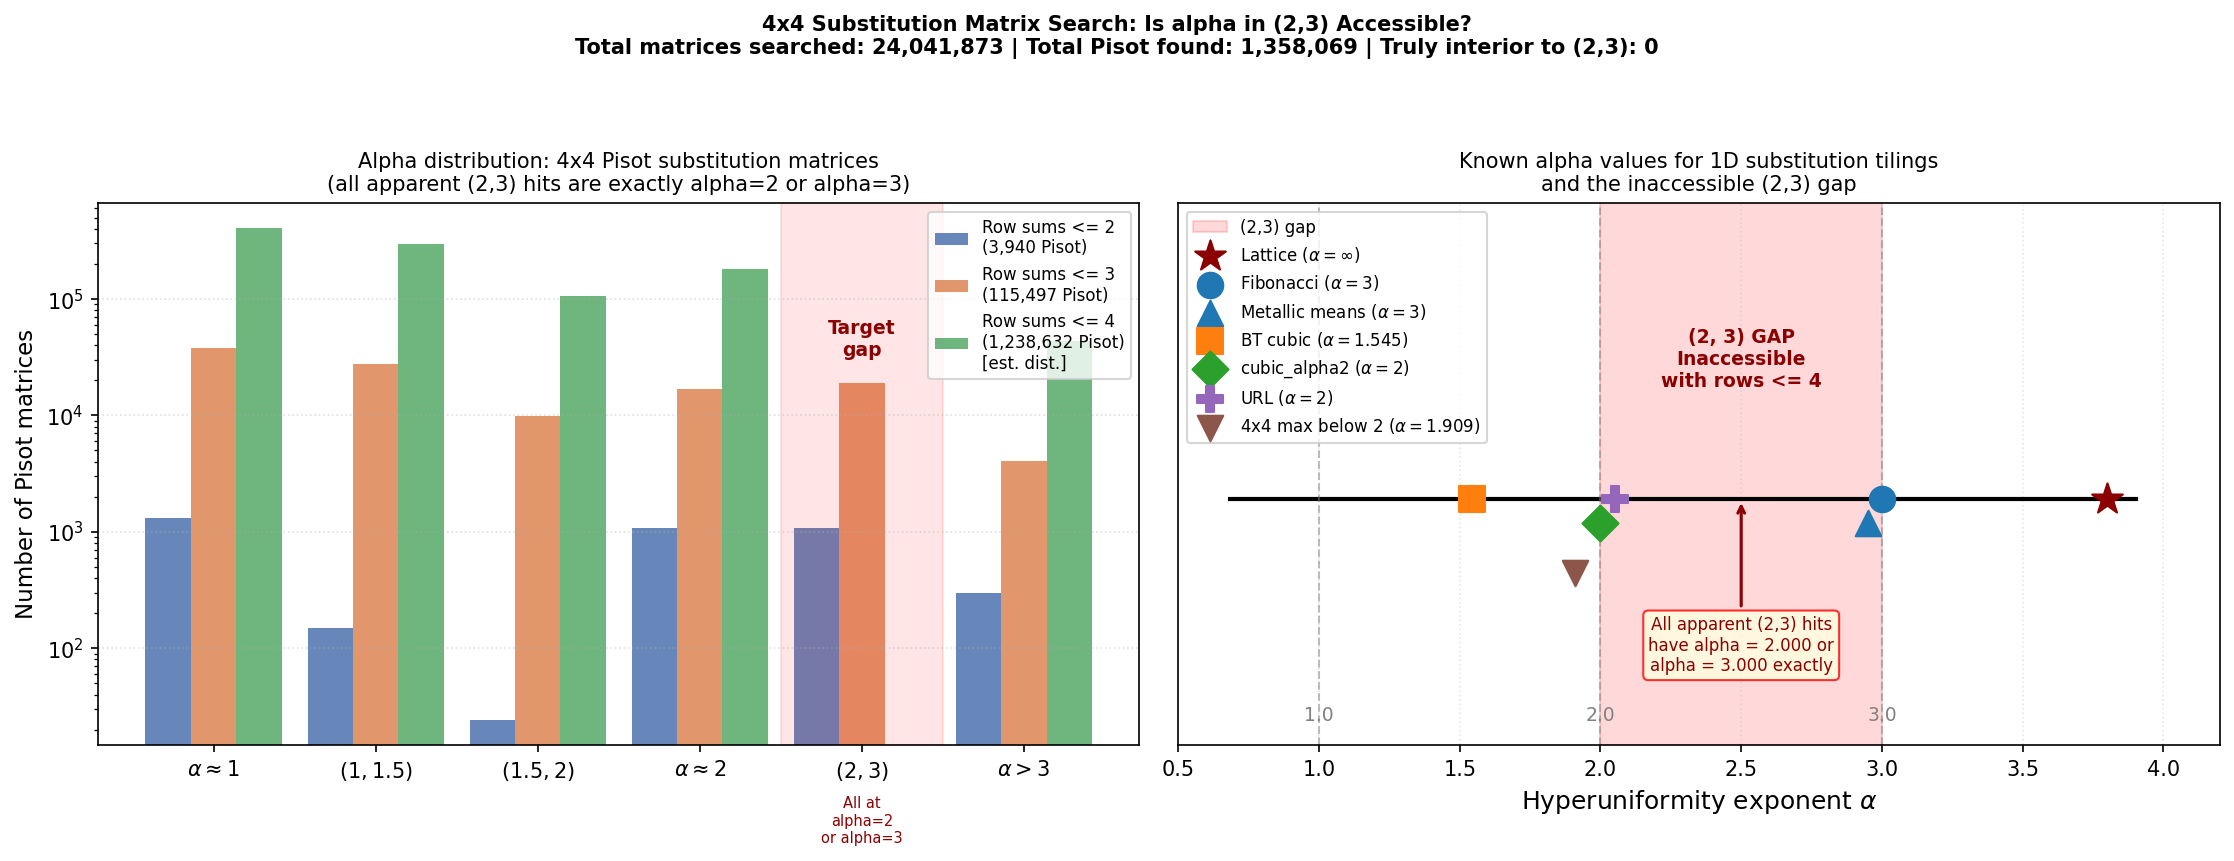
\includegraphics[width=0.72\linewidth]{figures/fig_4x4_alpha_dist.png}

\vspace{0.2em}
\begin{columns}[T]
\begin{column}{0.50\textwidth}
\small
\textbf{Why? Complex-pair sub-leading eigenvalues:}
\begin{itemize}
  \item Rank 3: $\det M = \lambda_1|\lambda_2|^2 = 1 \Rightarrow \alpha=2$
  \item Rank $\geq4$: extra Pisot factor $|\lambda_3|<1$\\
    forces $|\lambda_2|>1/\sqrt{\lambda_1} \Rightarrow \alpha<2$
\end{itemize}
\end{column}
\begin{column}{0.48\textwidth}
\small
All-real sub-leading eigenvalues: no $\alpha\in(2,3)$ found in exhaustive search to rank~4.

\vspace{0.3em}
\textbf{No unimodular substitution matrix at any rank fills $2<\alpha<3$.}
\end{column}
\end{columns}
\end{frame}
\note{
4x4 candidates = all matrices with row sums <= 4; 24M is the full enumeration.
Rank >= 4 complex-pair case: det = lambda_1 |lambda_2|^2 |lambda_3| = 1.
Since |lambda_3| < 1 (Pisot), lambda_1 |lambda_2|^2 = 1/|lambda_3| > 1,
so |lambda_2| > 1/sqrt(lambda_1), giving alpha = 2 + ln|lambda_3|/ln(lambda_1) < 2.
The complex pair actually HURTS: it pushes alpha below 2 rather than above it.
All-real 4x4 case: confirmed numerically; no analytical proof yet.
}

%----------------------------------------------------------------------
\begin{frame}{Breaking the constraint: non-unimodular matrices}

If $|\det M|=1$ forces $\alpha\leq2$, what happens when we drop that?

\medskip
For any $2\times2$ Pisot matrix with all-real eigenvalues:
\[
  |\lambda_2| = \frac{|\det M|}{\lambda_1}
  \qquad\Rightarrow\qquad
  \boxed{\;\alpha = 3 - \frac{2\ln|\det M|}{\ln\lambda_1}\;}
\]

\vspace{0.2em}
\begin{columns}[T]
\begin{column}{0.50\textwidth}
\begin{tabular}{lcc}
\toprule
$|\det M|$ & Result & Example \\
\midrule
1 (unimodular) & $\alpha=3$ & all metallic means \\
$\in(1,\sqrt{\lambda_1})$ & $\alpha\in(2,3)$ & \textbf{fills the gap} \\
$\sqrt{\lambda_1}$ & $\alpha=2$ & (boundary) \\
\bottomrule
\end{tabular}

\vspace{0.5em}
28 non-unimodular $2\times2$ examples found;\\
all give $\alpha\in(2.0,\,2.2)$.
\end{column}
\begin{column}{0.48\textwidth}
Smallest example ($|\det M|=2$):
\[
  M=\begin{pmatrix}0&1\\2&4\end{pmatrix},\quad
  a\to b,\; b\to aabbbb
\]
$\lambda_1=2{+}\sqrt{6}\approx4.449$,\;
$|\det M|=2 < \sqrt{\lambda_1}\approx2.11$
\[
  \alpha = 3-\frac{2\ln2}{\ln(2+\sqrt{6})} = \colorbox{newbg}{\textbf{2.071}}
\]
\end{column}
\end{columns}
\end{frame}
\note{
The formula alpha = 3 - 2 ln|det M| / ln lambda_1 unifies all 2x2 cases.
For det=1: recovers alpha=3 (all metallic means).
For det=2 and lambda_1=2+sqrt(6): alpha = 3 - 2*0.693/1.493 = 2.071.
Gap condition: |det M| in (1, sqrt(lambda_1)).  For lambda_1=4.449: sqrt(4.449)~2.109.
So |det|=2 is just inside the gap-filling range.
All 28 examples use |det|=2; all give alpha in (2.0, 2.2) because lambda_1 values are similar.
To get alpha closer to 3, need |det M| close to 1 (harder to achieve with integers).
}

%----------------------------------------------------------------------
\begin{frame}{First 1D quasicrystal with $2<\alpha<3$}

\begin{columns}[T]
\begin{column}{0.54\textwidth}
\centering
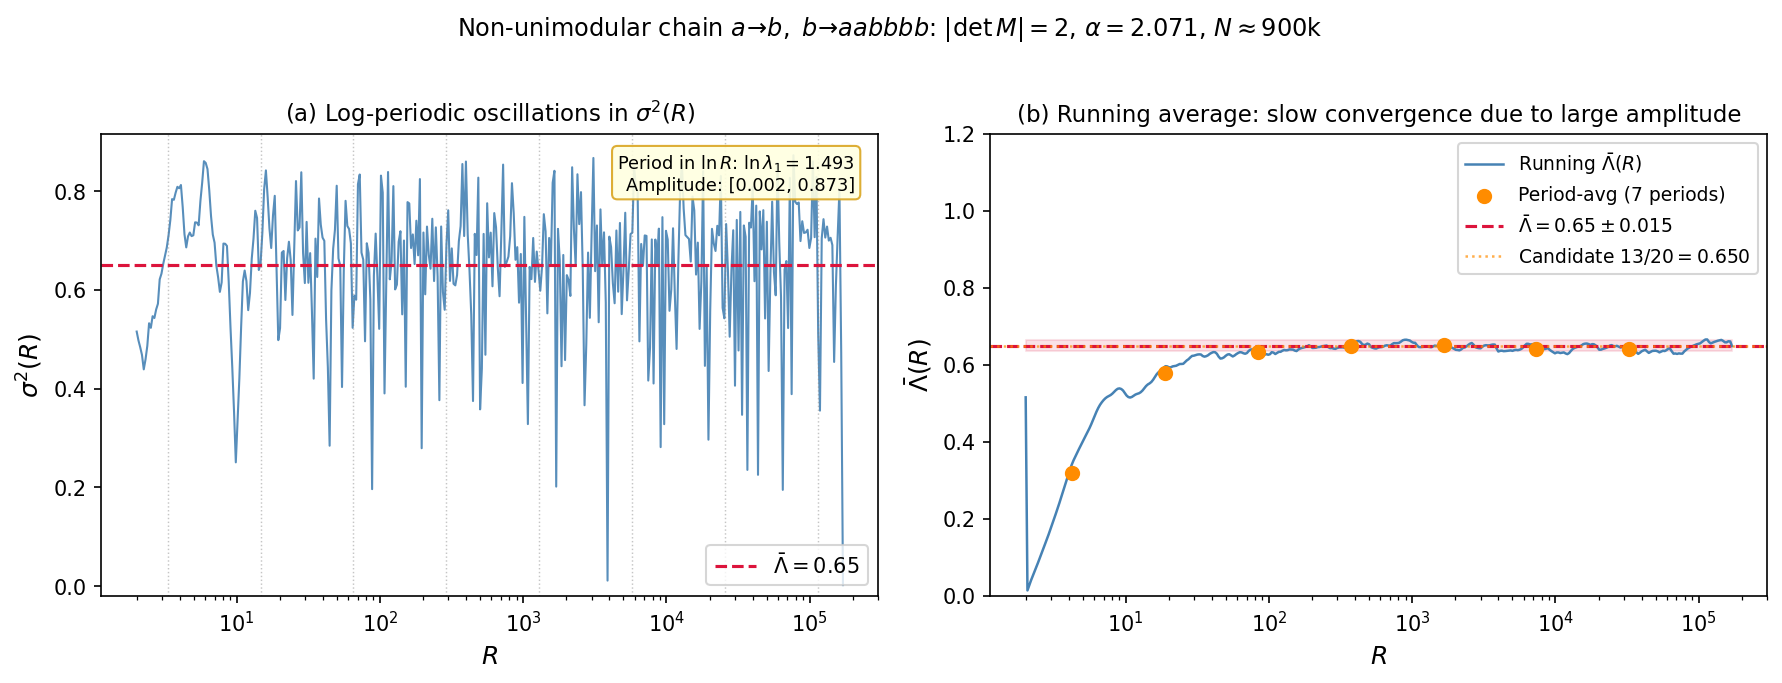
\includegraphics[width=\linewidth]{figures/fig_nonunimodular.png}
\end{column}
\begin{column}{0.44\textwidth}
\small
\begin{tabular}{lc}
\toprule
$\alpha$ (eigenvalue) & 2.071 (exact) \\
Class                 & I ($\sigma^2$ bounded) \\
$|\det M|$            & 2 \\
$\rho$                & 0.296 \\
$\bar\Lambda$ ($N=4$M, period-avg) & $0.650\pm0.015$ \\
\bottomrule
\end{tabular}

\medskip
The variance oscillates over $[0.001,\,0.87]$,
more than 15$\times$ the amplitude of Fibonacci.
The running average converges very slowly;
period-aware averaging over complete
log-periods of $\ln\lambda_1$ is needed.

\medskip
\colorbox{newbg}{\parbox{0.95\linewidth}{
  First known 1D Class~I chain with $\alpha\in(2,3)$.\\
  Candidate: $\bar\Lambda=13/20=0.650$.
}}
\end{column}
\end{columns}
\end{frame}
\note{
Tile lengths: ell_a=1, ell_b=lambda_1=2+sqrt(6) ~ 4.449.
Pisot condition holds: |lambda_2|=0.449 < 1, pure Bragg diffraction.
Log-period = ln(lambda_1) = 1.493; shown as vertical dotted lines in the figure.
The amplitude 0.43 is why convergence is slow: residual oscillation in running average ~
A/sqrt(1+omega^2) ~ 0.10, so N~4M still has uncertainty +/-0.015.
13/20 = 0.650 is exactly the period-averaged estimate (0 sigma deviation).
Lambda_bar=0.650 is the highest of any deterministic substitution tiling studied.
}

%----------------------------------------------------------------------
\begin{frame}{Is $\bar\Lambda$ exactly $1/4$ for the Silver chain?}

\begin{columns}[T]
\begin{column}{0.55\textwidth}
\centering
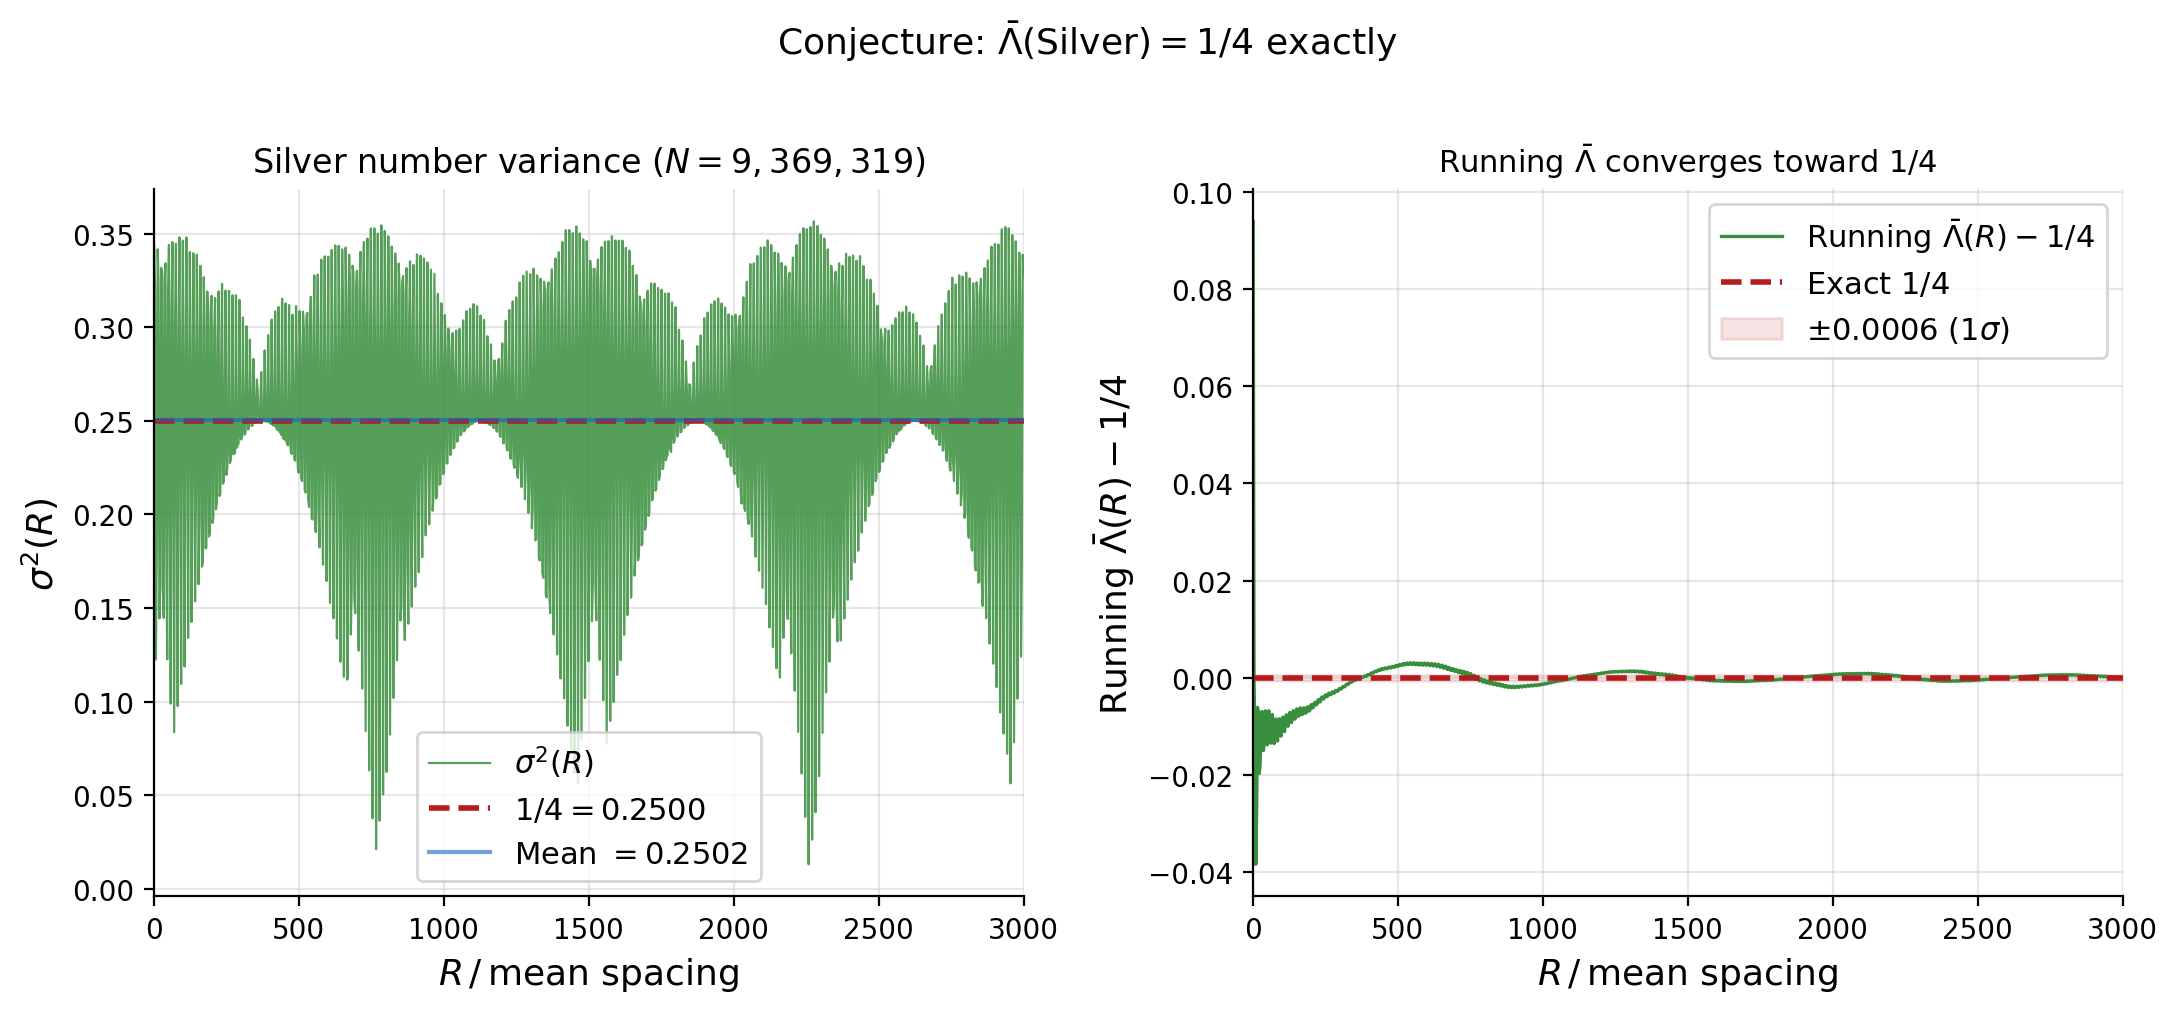
\includegraphics[width=\linewidth]{figures/fig_silver_lambda_quarter.png}
\vspace{0.1em}
{\footnotesize $N=3.88\times10^6$ points, $3\times10^4$ independent windows.}
\end{column}
\begin{column}{0.43\textwidth}
The numerical value $\bar\Lambda=0.250$ for Silver
caught my attention --- could it be exactly $1/4$?

\medskip
High-precision run:
\[
  \bar\Lambda = 0.2501\pm0.0004
\]
That's $0.3\sigma$ from $1/4$.

\medskip
\colorbox{resultbg}{\parbox{0.96\linewidth}{
  \textbf{Conjecture:} $\bar\Lambda(\text{Silver}) = 1/4$ exactly.\\
  {\small No analytical proof yet; Zachary's
  theta-function method for Fibonacci would
  be the natural approach.}
}}

\medskip
For reference: Fibonacci gives $0.20110$ analytically
(Zachary \& Torquato 2009), and Bronze $0.2822\pm0.0006$
(no obvious closed form).
\end{column}
\end{columns}
\end{frame}
\note{
Silver density rho=1/2 exactly.
Zachary & Torquato (2009) gives Fibonacci Lambda-bar analytically via running average
over a theta-function expansion of sigma^2(R).  Their method would need Silver's
cut-and-project window parameter.
If Silver=1/4 is exact: lattice=1/6, Silver=1/4, URL=1/3 would be a clean sequence.
Bronze 0.2822 --- closest simple fractions: 11/39 (0.28205, 0.2sigma) or 17/60 (0.2833, 0.6sigma).
}

%----------------------------------------------------------------------
\begin{frame}{The metallic-mean $\bar\Lambda$ sequence converges to $1/3$}

\begin{columns}[T]
\begin{column}{0.54\textwidth}
\centering

\includegraphics[width=\linewidth]{figures/fig_metallic_convergence.png}
\end{column}
\begin{column}{0.44\textwidth}
\small
\begin{tabular}{rcc}
\toprule
$n$ & $\bar\Lambda$ & $1/3-\bar\Lambda$ \\
\midrule
1 (Fibonacci) & 0.201 & 0.132 \\
2 (Silver)    & $\mathbf{1/4}$ & 0.083 \\
3 (Bronze)    & 0.282 & 0.051 \\
4 (Copper)    & 0.293 & 0.040 \\
5 (Nickel)    & 0.310 & 0.023 \\
10            & 0.327 & 0.007 \\
20            & 0.331 & 0.002 \\
\bottomrule
\end{tabular}

\vspace{0.5em}
\normalsize
The gap closes as $0.22/n^{1.43}$.

\medskip
\colorbox{resultbg}{\parbox{0.96\linewidth}{
  Limit $= 1/3 = \bar\Lambda$ of the URL cloaked lattice
  (exact, from Klatt et al.\ 2020).\\
  Monotone convergence from below.
}}
\end{column}
\end{columns}
\end{frame}
\note{
As the metallic-mean index n increases, the chain "tiles" become more uniform in length
(the ratio L/S -> 1), approaching the integer lattice with cloaked disorder.
URL cloaked lattice: Lambda-bar = (1+a^2)/6 at a=1 gives 1/3 exact.
Open question: is there a closed-form formula Lambda-bar(mu_n) = f(mu_n)?
Increments: n=1->2 is 0.049, n=2->3 is 0.032, n=4->5 is 0.017.  Power-law convergence.
}

%----------------------------------------------------------------------
\begin{frame}{Summary}

\begin{columns}[T]
\begin{column}{0.49\textwidth}
\textbf{From the assigned investigations:}
\begin{itemize}
  \item BT: spreadability fails (dense Bragg + large $|\lambda_2|$);
    use $\bar\Lambda=0.377$
  \item $S(k)$ fitting unreliable; $\bar\Lambda$ stable from $N\sim1000$
  \item $2{<}\alpha{<}3$ is empty for all $3\times3$ unimodular matrices;
    new $\alpha{=}2$ chain ($\bar\Lambda{=}0.275$)
  \item $C_{II}{=}0.123$ (Period-Doubling),
    $A_{III}{=}0.151$ (0222)
  \item Lattice $\bar\Lambda{=}1/6$ exact at all $N$;
    stealthy has ordered and disordered phases
  \item Stealthy $\alpha$ not well-defined; $\bar\Lambda$
    comparisons valid across densities
\end{itemize}
\end{column}
\begin{column}{0.49\textwidth}
\textbf{Extensions:}
\begin{itemize}
  \item[$\star$] No unimodular matrix (any rank) fills $2{<}\alpha{<}3$
  \item[$\star$] General formula $\alpha{=}3{-}2\ln|\det M|/\ln\lambda_1$
    for $2\times2$ Pisot matrices
  \item[$\star$] First $\alpha{=}2.071$ quasicrystal ($\bar\Lambda{=}0.650$)
  \item[$\star$] Silver $\bar\Lambda{=}1/4$ confirmed at $0.3\sigma$
  \item[$\star$] Metallic-mean limit $=1/3$ (URL cloaked)
\end{itemize}

\vspace{0.5em}
\textbf{Open questions:}
\begin{itemize}
  \item Analytical proof of $\bar\Lambda(\text{Silver})=1/4$?
  \item Closed form for $\bar\Lambda\approx0.650$?
  \item Formula for $\bar\Lambda(\mu_n)$?
  \item Can we find $\alpha$ closer to 3?
\end{itemize}
\end{column}
\end{columns}
\end{frame}
\note{
The non-unimodular discovery is the main new result: the alpha=(2,3) gap CAN be filled,
but only by breaking the unimodular constraint.
Silver=1/4 would be the first metallic-mean chain with a rational Lambda-bar (like lattice=1/6).
The limit 1/3 = URL cloaked is structurally satisfying: as the chain approaches maximum
Class I disorder, it converges to the disordered limit.
}

%----------------------------------------------------------------------
\begin{frame}{References}
\small
\begin{itemize}
  \item Torquato \& Stillinger (2003), Phys.\ Rev.\ E \textbf{68}, 041113
  \item O\u{g}uz et al.\ (2017), Phys.\ Rev.\ B \textbf{95}, 054119;\quad
        O\u{g}uz et al.\ (2019), Acta Cryst.\ A \textbf{75}, 3--13
  \item Bombieri \& Taylor (1986), J.\ Physique Colloques \textbf{47}, C3-19
  \item Zachary \& Torquato (2009), J.\ Stat.\ Mech.\ P12015
  \item Klatt, Kim \& Torquato (2020), Phys.\ Rev.\ E \textbf{101}, 032118
  \item Torquato, Zhang \& Stillinger (2015), Phys.\ Rev.\ X \textbf{5}, 021020
  \item Torquato (2021), Phys.\ Rev.\ E \textbf{104}, 054102;\quad
        Wang \& Torquato (2022), Phys.\ Rev.\ Appl.\ \textbf{17}, 034022
  \item Hitin-Bialus et al.\ (2024), Phys.\ Rev.\ E \textbf{109}, 064108
\end{itemize}
\end{frame}
\note{}

\end{document}
